\subsection{Wytworzone oprogramowanie}

Modularność projektu sprawia, że wygodniej jest omówić niezależnie każdą z części. Dla jasności, przebieg całego procesu jest przedstawiony na schemacie \ref{fig:przebieg_procesu}. Każda funkcjonalność, jak i wizualizacje wyników poszczególnych zadań są dostępne poprzez interfejs użytkownika. 

\begin{figure}[!h]
    \centering
    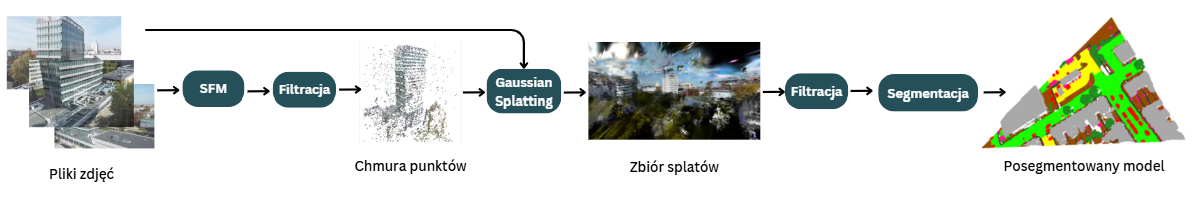
\includegraphics[width=1.0\linewidth]{images/przebieg.png}
    \caption{Przebieg procesu}
    \label{fig:przebieg_procesu}
\end{figure}